%%%%%%%%%%%%%%%%%%%%%%%%%%%%%%%%%%%%%%%%%%%%%%%%%%%%
% LECTURE 13
%%%%%%%%%%%%%%%%%%%%%%%%%%%%%%%%%%%%%%%%%%%%%%%%%%%%
\subsection*{Nusselt Number and Heat Transfer Coefficients over a Flat Plate}
\addcontentsline{toc}{subsection}{Nusselt Number and Heat Transfer Coefficients over a Flat Plate}
%%%%%%%%%%%%%%%%%%%%%%%%%%%%%%%%%%%%%%%%%%%%%%%%%%%%%%%%%%%

For a flow over a flat plate, the local heat transfer can be determined by examining the solution at the surface. Since the fluid velocity at the wall is zero (no-slip condition), heat transfer at the surface reduces to conduction:

\[
    q_s'' = -k\left.\frac{\partial T}{\partial y}\right|_{y=0} = h_x (T_s - T_\infty)
\]
\begin{definition}
    \[
            h_x = \frac{-k\left.\frac{\partial T}{\partial y}\right|_{y=0}}{T_s - T_\infty}\ \qquad \textit{,flow over a flat surface}
    \]
\end{definition}
%
The Nusselt number is defined as:
\begin{definition}
\[
    \text{Nu}_x =  \frac{h_x \cdot x}{k_f} = f(x^*,\operatorname{Re_L}, \operatorname{Pr}) = \frac{\text{convective heat transfer}}{\text{conductive heat transfer}}
\]
\end{definition}
%
Where:
\begin{itemize}
    \item $h$ is the local heat transfer coefficient
    \item $x$ is the distance from the leading edge
    \item $k_f$ is the thermal conductivity of the fluid
\end{itemize}

\textit{Physical meaning:} The Nusselt number represents the ratio of convective heat transfer to conductive heat transfer. It indicates the enhancement of heat transfer due to convection relative to conduction across the same fluid layer.

%%%%%%%%%%%%%%%%%%%%%%%%%%%%%%%%%%%%%%%%%%%%%%%%%%%%%%%%%%%
\subsubsection*{Average Nusselt Number}
\addcontentsline{toc}{subsubsection}{Average Nusselt Number}

The average Nusselt number over a length $L$ is defined as:
\begin{definition}
    \[
        \overline{\text{Nu}} = \frac{\bar{h}\cdot L}{k_f} = f(\operatorname{Re_L}, \operatorname{Pr})
    \]
\end{definition}
%
where
\begin{definition}
    \[
        \overline{h} = \frac{1}{L}\int_0^L \,h_x\,dx
    \]
\end{definition}
%
\textit{Note:} If we know Nu, we can find $h$. All relationships can be found in table 7.7 and 8.4 of textbook.
\\[0.5em]
\textit{Warning:} It's important to note that the average Nusselt number is not the average of local Nusselt numbers. Rather, it's defined using the average heat transfer coefficient:
\[
    \overline{\text{Nu}} \neq \frac{1}{L}\int_0^L\operatorname{Nu}_x \,dx
\]


%%%%%%%%%%%%%%%%%%%%%%%%%%%%%%%%%%%%%%%%%%%%%%%%%%%%%%%%%%%
\subsection*{Mass Transfer: Sherwood Number}
\addcontentsline{toc}{subsection}{Mass Transfer: Sherwood Number}
% Similarly for mass transfer
% \[
%        C_f=\frac{2}{\operatorname{Re_L}} f\left(x^*, \operatorname{Re_L}\right)=\left.\frac{2}{\operatorname{Re_L}} \frac{\partial u^*}{\partial y^*}\right|_{y^*=0} 
% \]
We can define a similar dimensionless parameter called the Sherwood number:
\[
    \text{Sh}_x = \frac{h_m\cdot x}{D_{AB}} = \frac{\partial C^*_A}{\partial y^*} \Bigl \vert_{y^* =0} = \frac{\text{Convective mass transfer}}{\text{Diffusive mass transfer}}
\]

Where:
\begin{itemize}
    \item $h_m$ is the mass transfer coefficient [m/s]
    \item $D_{AB}$ is the binary diffusion coefficient [m²/s]
\end{itemize}

The average Sherwood number is defined as:
\[
\overline{\text{Sh}} = \frac{\bar{h}_m L}{D_{AB}}
\]
%%%%%%%%%%%%%%%%%%%%%%%%%%%%%%%%%%%%%%%%%%%%%%%%%%%%%%%%%%%
\subsection*{Heat and Mass Transfer Analogy}
\addcontentsline{toc}{subsection}{Heat and Mass Transfer Analogy}

Thermal boundary layers and concentration boundary layers have identical forms by replacing
\begin{itemize}
    \item $\text{Pr} \rightarrow \text{Sc}$
    \item $\text{Nu} \rightarrow \text{Sh}$
\end{itemize}
%
\textit{Example: } For laminar flow over a flat plate with $\operatorname{Pr} \ge 0.6$, we have
\[
        \operatorname{Nu_x} = 0.332 \, \operatorname{Re_x}^{1/2}\,\operatorname{Pr}^{1/3}
\]
for the same type flow, we can say
\[
        \operatorname{Sh_x} = 0.332 \, \operatorname{Re_x}^{1/2}\,\operatorname{Sc}^{1/3}
\]
In general, for boundary \textit{laminar} layer flows, Nusselt and Sherwood numbers follow the form:
\[
    \text{Nu} \sim f(x^*, \operatorname{Re_L})\,\text{Pr}^n \sim \operatorname{Re_L}^m\, \operatorname{Pr}^n 
\]
\[
\text{Sh} \sim f(x^*, \operatorname{Re_L})\, \text{Sc}^n \sim  \operatorname{Re_L}^m\, \operatorname{Sc}^n 
\]

This leads to the relationship:
\[
\frac{\text{Nu}}{\text{Sh}} \approx \left(\frac{\text{Pr}}{\text{Sc}}\right)^n \approx Le^{-n}
\]

The ratio $\frac{\text{Sc}}{\text{Pr}}$ is known as the Lewis number ($\text{Le}$):
\[
\text{Le} = \frac{\text{Sc}}{\text{Pr}} = \frac{\nu/D_{AB}}{\nu/\alpha} = \frac{\alpha}{D_{AB}} 
\]

For most boundary layer flows, $n \approx 1/3$, which leads to:
\[
    \frac{\text{Nu}}{\text{Sh}} \approx \left(\frac{\text{Pr}}{\text{Sc}}\right)^{1/3} = \text{Le}^{-1/3}
\]

Similarly, the ratio of boundary layer thicknesses follows:
\[
\frac{\delta_t}{\delta_C} \approx \left(\frac{\text{Sc}}{\text{{Pr}}}\right)^n = \text{Le}^{n}
\]
%
It can be shown that
\[
    \frac{h}{h_m}=\rho\, c_p L_e^{1-n}=\frac{k}{D_{AB}\, L_e^n}
\]
% %%%%%%%%%%%%%%%%%%%%%%%%%%%%%%%%%%%%%%%%%%%%%%%%%%%%%%%%%%%
% \subsubsection*{Example: Shaving Pets}
% \addcontentsline{toc}{subsubsection}{Example: Shaving Pets}

% A common misconception is that shaving pets (like dogs or cats) helps them stay cool in hot weather. Let's analyze this from a heat/mass transfer perspective:

% \begin{itemize}
%     \item If ambient temperature exceeds body temperature ($T_\infty > T_\text{body}$), shaving fur actually increases heat transfer \textit{into} the animal's body
%     \item Unlike humans, most pets don't cool through sweating (no mass transfer via evaporation from skin)
%     \item Pets primarily cool through panting and breathing (evaporative cooling in lungs)
%     \item For example, a golden retriever has a lung surface area of approximately 50 m²
% \end{itemize}

% Correct approach: Keep the fur (insulation) and provide plenty of water to enable cooling through respiration.

%%%%%%%%%%%%%%%%%%%%%%%%%%%%%%%%%%%%%%%%%%%%%%%%%%%%%%%%%%%
% \subsection*{Similarity Solutions for Laminar Boundary Layer Over a Flat Plate}
% \addcontentsline{toc}{subsection}{Similarity Solutions for Laminar Boundary Layer Over a Flat Plate}

% Experimental observations show that velocity profiles at different positions along a flat plate have similar shapes when properly scaled. This suggests a similarity solution approach.
% %
    
% %
% We introduce a similarity variable:
% \[
% \eta = y\sqrt{\frac{U_\infty}{\nu x}}
% \]

% And define a stream function $\psi$ such that:
% \[
% u = \frac{\partial \psi}{\partial y}, \quad v = -\frac{\partial \psi}{\partial x}
% \]

% The stream function is expressed as:
% \[
% \psi = \sqrt{\nu U_\infty x} \, f(\eta)
% \]

% Substituting into the boundary layer equations leads to an ordinary differential equation (ODE):
% \[
% f''' + \frac{1}{2}ff'' = 0
% \]

% With boundary conditions:
% \[
% f(0) = 0, \quad f'(0) = 0, \quad f'(\infty) = 1
% \]

% This nonlinear ODE does not have a closed-form analytical solution. It must be solved numerically using a "shooting method" approach:

% \begin{enumerate}
%     \item Guess a value for $f''(0)$
%     \item Integrate from $\eta = 0$ using this initial condition
%     \item Check if $f'(\infty) = 1$ is satisfied
%     \item If not, adjust the guess for $f''(0)$ and repeat
% \end{enumerate}

% From the numerical solution, we obtain:
% \begin{itemize}
%     \item The velocity boundary layer thickness: $\delta \approx \frac{5}{\sqrt{\text{Re}_x}} x$
%     \item The skin friction coefficient: $C_f = \frac{\tau_w}{\frac{1}{2}\rho U_\infty^2} = \frac{0.664}{\sqrt{\text{Re}_x}}$
%     \item The average skin friction coefficient: $\overline{C}_f = \frac{1.328}{\sqrt{\text{Re}_L}} = 2C_f|_{x=L}$
% \end{itemize}

% %%%%%%%%%%%%%%%%%%%%%%%%%%%%%%%%%%%%%%%%%%%%%%%%%%%%%%%%%%%
% \subsubsection*{Thermal Boundary Layer Solution}
% \addcontentsline{toc}{subsubsection}{Thermal Boundary Layer Solution}

% With the velocity field determined, we can solve for the thermal boundary layer using a similar approach. We define a dimensionless temperature:
% \[
% \theta = \frac{T - T_s}{T_\infty - T_s}
% \]

% The energy equation becomes:
% \[
% \theta'' + \frac{\text{Pr}}{2}f\theta' = 0
% \]

% With boundary conditions:
% \[
% \theta(0) = 0, \quad \theta(\infty) = 1
% \]

% This is a linear ODE that can be solved once $f(\eta)$ is known. The solution depends on the Prandtl number.

% The temperature gradient at the wall gives the Nusselt number:
% \[
% \text{Nu}_x = -\theta'(0)\sqrt{\text{Re}_x}
% \]

% The value of $\theta'(0)$ depends on Pr:
% \begin{itemize}
%     \item For $0.6 \leq \text{Pr} \leq 10$: $\theta'(0) \approx -0.332 \, \text{Pr}^{1/3}$
%     \item For $\text{Pr} \ll 0.1$ (e.g., liquid metals): $\theta'(0) \approx -0.565 \, \text{Pr}^{1/2}$
%     \item For $\text{Pr} > 10$ (e.g., oils): $\theta'(0) \approx -0.0339 \, \text{Pr}^{1/3}$
% \end{itemize}

% This leads to the following correlations:
% \[
% \text{Nu}_x = \begin{cases}
% 0.332 \, \text{Re}_x^{1/2} \, \text{Pr}^{1/3}, & 0.6 \leq \text{Pr} \leq 10 
% \\[1em]
% 0.565 \, \text{Re}_x^{1/2} \, \text{Pr}^{1/2}, & \text{Pr} \ll 0.1 
% \\[1em]
% 0.0339 \, \text{Re}_x^{1/2} \, \text{Pr}^{1/3}, & \text{Pr} > 10
% \end{cases}
% \]

% For the average Nusselt number:
% \[
% \overline{\text{Nu}}_L = \frac{1/L \int_0^Lq''_s dx}{Ts-T_\infty}\cdot\frac{L}{k_f} =2 \, \text{Nu}_x\Bigl|_{x=L}
% \]
%%%%%%%%%%%%%%%%%%%%%%%%%%%%%%%%%%%%%%%%%%%%%%%%%%%%%%%%%%%
% Combined Lecture Notes on Laminar Boundary Layer Similarity Solutions
% Merging the user’s notes, professor’s transcribed explanation, and professor’s notes.
%%%%%%%%%%%%%%%%%%%%%%%%%%%%%%%%%%%%%%%%%%%%%%%%%%%%%%%%%%%

\subsection*{Similarity Approach for Laminar Boundary Layer Over a Flat Plate}
\addcontentsline{toc}{subsection}{Similarity Approach for Laminar Boundary Layer Over a Flat Plate}
%%%%%%%%%%%%%%%%%%%%%%%%%%%%%%%%%%%%%%%%%%%%%%%%%%%%%%%%%%%

From experimental observations, velocity profiles at different locations along a flat plate can be made to collapse into a single curve when properly scaled in the boundary-layer region. This suggests a similarity solution approach:
\[
  u = f(y\cdot g(x)) = f(\eta),
\]
where we define the similarity variable \(\eta\) to capture the dependence on both \(x\) and \(y\).

\bigskip
 \textbf{Governing Equations (Boundary Layer Approximation):}
\begin{align*}
  u\frac{\partial u}{\partial x} + v\frac{\partial u}{\partial y} &= \nu \frac{\partial^2 u}{\partial y^2}, \\
  \frac{\partial u}{\partial x} + \frac{\partial v}{\partial y} &= 0.
\end{align*}

 \textbf{Stream Function:}\
We introduce the stream function \(\psi\) such that:
\[
  u = \frac{\partial \psi}{\partial y}, \quad v = -\frac{\partial \psi}{\partial x}.
\]
This identically satisfies the continuity equation.

\bigskip
 \textbf{Similarity Variables:}\
We choose:
\[
  \psi(x,y) = \sqrt{\nu U_\infty x}\, f(\eta), \quad\text{where}\quad \eta = y \sqrt{\frac{U_\infty}{\nu x}}.
\]
Then,
\[
  u = \frac{\partial \psi}{\partial y} = \left( f'(\eta)\,\sqrt{\nu U_\infty x} \right)\!\left(\sqrt{\frac{U_\infty}{\nu x}} \right) = U_\infty\, f'(\eta),
\]
\[
  v = -\frac{\partial \psi}{\partial x} = -\frac{d}{dx}\Bigl(\sqrt{\nu U_\infty x}\, f(\eta)\Bigr).
\]
One can show:
\[
  v = \frac{1}{2}\sqrt{\frac{\nu U_\infty}{x}}\bigl(\eta f'(\eta) - f(\eta)\bigr) = U_\infty\,\sqrt{\frac{\nu}{U_\infty x}}\,\frac{\eta f' - f}{2} = Re^{-1/2}_x\,\frac{\eta f' - f}{2},
\]
where \( Re_x = \frac{U_\infty x}{\nu}\) is the Reynolds number based on distance \(x\).

\paragraph{Substituting into the Momentum Equation: }
By carefully differentiating and substituting into 
\[
  u \frac{\partial u}{\partial x} + v\frac{\partial u}{\partial y} = \nu \frac{\partial^2 u}{\partial y^2}
\]
one obtains the ordinary differential equation:
%
\[
  f'''+\frac{1}{2} f f'' = 0 \quad\text{or equivalently}\quad f f'' + 2f'''=0.
\]
This is a nonlinear ODE with boundary conditions:
%
\[
  f(0)=0,\quad f'(0)=0,\quad f'(\infty)=1.
\]
%
 Because it is nonlinear, a classic approach is the ``shooting method''\,:
\begin{enumerate}
  \item Guess \( f''(0) \) at \(\eta=0\).
  \item Integrate numerically in \(\eta\) from 0 to some large value.
  \item Check if \( f'(\infty)=1 \). If not, adjust \( f''(0) \) and repeat.
\end{enumerate}
%
\paragraph{Solutions and Key Results:}
\begin{itemize}
    \item At \(\eta\approx 5.0\), the velocity \(u\approx 0.99\,U_\infty\). This defines the boundary-layer thickness:
    \[
      \delta \approx 5\sqrt{\frac{\nu x}{U_\infty}}\quad\Rightarrow\quad \frac{\delta}{x} = \frac{5}{\sqrt{Re_x}}.
    \]
    %
    \item The local friction coefficient \( C_{f,x}\) is given by:
    \[
      C_{f,x} = \frac{\tau_{w}}{\frac{1}{2}\rho U_\infty^2}
    \]
    where 
    \[
        \tau_w = \mu\frac{\partial u}{\partial y}\Bigr\rvert_{y=0} = \mu\left[ U_\infty f''(0)\sqrt{\frac{U_\infty}{\nu x}}\right]
    \]
    Numerically, \(f''(0)\approx 0.332\), so:
    \[
      C_{f,x} = \frac{0.664}{\sqrt{Re_x}}
    \]
    %
    \item The average friction coefficient over a plate of length \(L\) is \(\overline{C}_{f} = 2\,C_{f,x}\bigl|_{x=L}\)
    %
    \item $\operatorname{Re} \uparrow\, \Leftrightarrow \, \delta \downarrow \,\Leftrightarrow \, u_\infty \uparrow$
\end{itemize}
%
\begin{figure}[H]
    \centering
    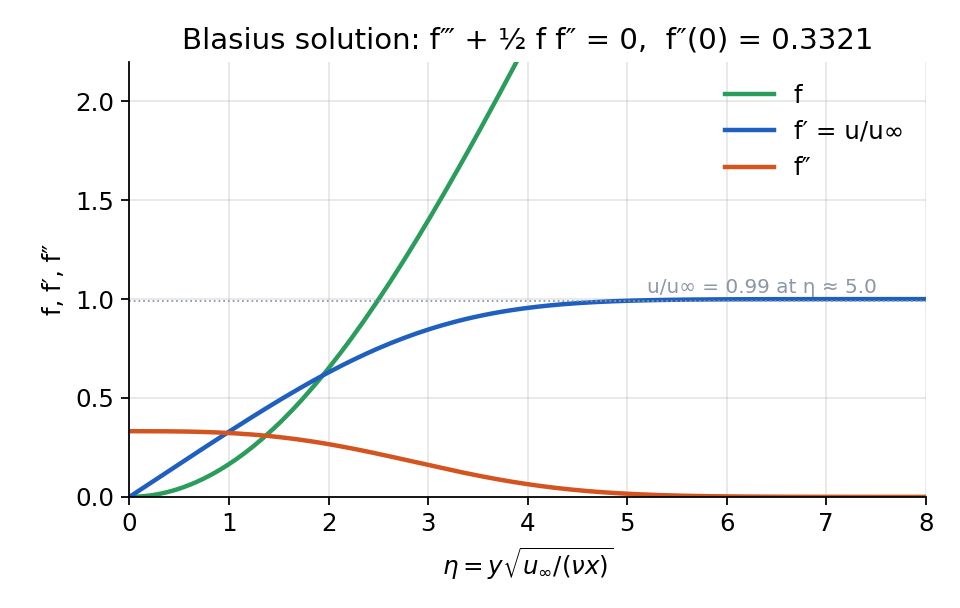
\includegraphics[width=0.65\linewidth]{pics/Belasisus_sol.png}
    \caption{Belasius solution.}
\end{figure}

The figure is computed, not copied; the whole solution is a shooting problem on $f''(0)$:
\begin{lstlisting}[language=Python]
import numpy as np
from scipy.integrate import solve_ivp
from scipy.optimize import brentq

def blasius(s):                       # integrate f''' = -f f''/2 from a guess s = f''(0)
    rhs = lambda eta, y: [y[1], y[2], -0.5 * y[0] * y[2]]
    return solve_ivp(rhs, [0, 10], [0, 0, s], rtol=1e-9)

s = brentq(lambda s: blasius(s).y[1, -1] - 1, 0.2, 0.5)   # choose s so that f'(inf) = 1
print(f"f''(0) = {s:.4f}")                                 # 0.3321
\end{lstlisting}


%%%%%%%%%%%%%%%%%%%%%%%%%%%%%%%%%%%%%%%%%%%%%%%%%%%%%%%%%%%
\subsection*{Similarity Approach for Thermal Boundary Layer Over A Flat Plate}
\addcontentsline{toc}{subsection}{Similarity Approach for Thermal Boundary Layer Over A Flat Plate}
%%%%%%%%%%%%%%%%%%%%%%%%%%%%%%%%%%%%%%%%%%%%%%%%%%%%%%%%%%%
Thermal Energy Equation for a Flat Plate is as follows:
%
\begin{align*}
  u\frac{\partial T}{\partial x} + v\frac{\partial T}{\partial y} = \alpha\,\frac{\partial^2 T}{\partial y^2},
\end{align*}
where \(\alpha = k/(\rho c_p)\) is the thermal diffusivity. Define the dimensionless temperature:
\[
  T^* = \theta = \frac{T - T_s}{T_\infty - T_s},\quad 0 \le \theta \le 1,
\]
with boundary conditions:
\[
    \begin{array}{ll}
        y =0, &  \theta = 0\\
        y = \infty, & \theta = 1\\
        x =0,  & \theta = 1
    \end{array}
\]
%
\paragraph{Similarity Form of the Energy Equation:}
Using 
\[
    \eta = y\sqrt{\frac{U_\infty}{\nu x}}
\]
same as velocity boundary layer and the known function \(f(\eta)\) from the velocity solution, the dimensionless energy equation becomes:
\[
  \theta''(\eta) + \frac{\operatorname{Pr}}{2}\,f(\eta)\,\theta'(\eta) = 0,\quad \text{where}
  \quad 
  \operatorname{Pr} = \frac{\nu}{\alpha}
\]
 The boundary conditions are \(\theta(0)=0\) and \(\theta(\infty)=1\). Unlike the velocity ODE, this is linear in \(\theta\), but it depends on \(f(\eta)\) which is only known numerically.

\paragraph{Integral Form of the Solution:}\
One can find the solution as follow:
\[
    \theta(\eta)=C_1 \int_0^\eta \exp \left(\frac{\operatorname{Pr}}{2} \int_0^{\eta^{\prime \prime}} f\left(\eta^{\prime}\right) d \eta^{\prime}\right) d \eta^{\prime} + C_2
\]
where $\eta^{\prime}$ and $\eta^{\prime \prime}$ are dummy variables. Apply BCs, we'll get
\[
  \theta(\eta) = \frac{\displaystyle\int_0^{\eta} \exp\!\Bigl(-\frac{\operatorname{Pr}}{2}\int_0^{\eta''} f(\eta')\,d\eta'\Bigr) d\eta''}{\displaystyle\int_0^{\infty} \exp\!\Bigl(-\frac{\operatorname{Pr}}{2}\int_0^{\eta''} f(\eta')\,d\eta'\Bigr) d\eta''},
\]
In practice, one integrates numerically once \(f(\eta)\) is known.
%
\begin{figure}[H]
    \centering
    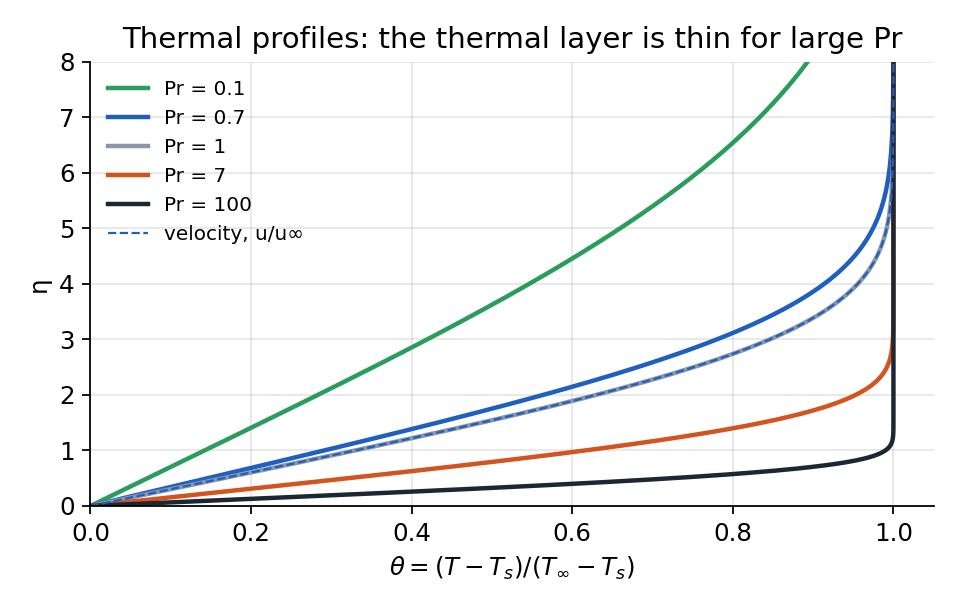
\includegraphics[width=0.7\linewidth]{pics/thermal_profile_flat_plate.png}
    \caption{Thermal profile solution}
\end{figure}
%
\paragraph{Local Heat Transfer Coefficient}\
Let \( q''_s = -k\bigl(\partial T/\partial y\bigr)_{y=0}\). Then,
\begin{align*}
    q''_s &= -k\biggl.\frac{\partial T}{\partial y}\biggr|_{y=0}\! \\\
    &= -k\,(T_\infty - T_s)\,\biggl.\frac{\partial \theta}{\partial y}\biggr|_{y=0}
    \\
    &= k\,(T_s - T_\infty)\,\biggl.\frac{\partial \theta}{\partial \eta}\biggr|_{\eta=0}\,\frac{\partial \eta}{\partial y}\bigg|_{y=0} 
    \\
    & = k\,(T_s - T_\infty)\,\,\sqrt{\frac{U_\infty}{\nu x}} \theta'(0)
\end{align*}
%
\begin{definition}
\paragraph{Nusselt Number (laminar flow)} Using local heat transfer coefficient, we can derive an expression for Nusselt number as follow:
\[
  h_x = \frac{q''_s}{T_s - T_\infty},\quad\text{and}\quad\text{Nu}_x = \frac{h_x\,x}{k} = \theta'(0)\,\sqrt{\text{Re}_x}.
\]
%
Numerical values of \(\theta'(0) = f(\operatorname{Pr})\). For typical ranges:
%
\[
    \left\{\begin{array}{rll}
         0.6 \le \operatorname{Pr} < 10: &  \theta'(0)\approx 0.332\,\operatorname{Pr}^{1/3}, & \text{Nu}_x = 0.332\,\text{Re}_x^{1/2}\,\operatorname{Pr}^{1/3}
         \\[1em]
         \operatorname{Pr} < 0.05: & \theta'(0)\approx 0.565\,\operatorname{Pr}^{1/2}, & \text{Nu}_x = 0.565\,\text{Re}_x^{1/2}\,\operatorname{Pr}^{1/2}
         \\[1em]
         \operatorname{Pr} > 10: & \theta'(0)\approx 0.0339\,\operatorname{Pr}^{1/3}, & \text{Nu}_x = 0.339\,\text{Re}_x^{1/2}\,\operatorname{Pr}^{1/3}
    \end{array}
    \right.
\]
\end{definition}

%
\paragraph{Average Nusselt Number:}
Analogous to the friction coefficient, one obtains:
\begin{definition}
    \[
      \overline{\text{Nu}}_L = \frac{\overline{h}\cdot L}{k_f}=2\,\text{Nu}_x\Bigl|_{x=L} = 2\,\theta'(0)\,\sqrt{\text{Re}_L}
      \qquad \overline{h} = 2 h
    \]
\end{definition}
%%%%%%%%%%%%%%%%%%%%%%%%%%%%%%%%%%%%%%%%%%%%%%%%%%%%%%%%%%%
\subsubsection*{Boundary Layer Thickness Ratio}
\addcontentsline{toc}{subsubsection}{Boundary Layer Thickness Ratio}
%%%%%%%%%%%%%%%%%%%%%%%%%%%%%%%%%%%%%%%%%%%%%%%%%%%%%%%%%%%
The ratio of thermal to velocity boundary layer thickness depends on the Prandtl number:
\[
\frac{\delta_t}{\delta} \approx \begin{cases}
\text{Pr}^{-1/3}, & \operatorname{Pr} > 0.6 
\\[1em]
\text{Pr}^{-1/2}, & \operatorname{Pr} \ll 0.1
\end{cases}
\]

This means:
\begin{itemize}
    \item For Pr > 1 (e.g., water, oils): $\delta_t < \delta$ (thermal boundary layer is thinner)
    \item For Pr = 1: $\delta_t = \delta$ (boundary layers are equal)
    \item For Pr < 1 (e.g., liquid metals): $\delta_t > \delta$ (thermal boundary layer extends beyond velocity boundary layer)
\end{itemize}
%%%%%%%%%%%%%%%%%%%%%%%%%%%%%%%%%%%%%%%%%%%%%%%%%%%%%%%%%%%
\subsection*{Mass Transfer Boundary Layers Solution}
\addcontentsline{toc}{subsection}{Mass Transfer Boundary Layers Solution}
%%%%%%%%%%%%%%%%%%%%%%%%%%%%%%%%%%%%%%%%%%%%%%%%%%%%%%%%%%%
We'll get the similar solution for mass transfer. Particularly,
\[
        \frac{\delta_c}{\delta} = \operatorname{Sc}^{-1/3}
\]
%
Unlike the Prandtl number, which spans several orders of magnitude ($10^{-2}$ to $10^5$), the Schmidt number typically has a narrower range:
%
\begin{table}[H]
    \centering
    \caption{Schmidt number for different oxygen, methanol, and Ammonia in air or water}
    \begin{tabular}{c|c|c} 
        & Air & Water \\
        \hline $\mathrm{O}_2$ & 0.99 & 441 \\
        Mehanal & 1.14 & 540 \\
        Ammonia & 0.57 & 360
    \end{tabular}
\end{table}
%
For quick estimates:
\begin{itemize}
    \item Gas diffusion: $Sc \approx 1$
    \item Liquid diffusion: $Sc \approx 100-500$
\end{itemize}

This difference occurs because liquids have much higher density and smaller mean free paths between molecular collisions, significantly impeding diffusion.
